\chapter{Design}
	
	% TODO: Past tenseify!
	
	In this chapter a system design is proposed based on the considerations of the
	previous chapter. An overview is given which is followed by a more detailed
	description of the important components of the system.
	
	\section{Overview}
		
		The 3D Printing system can be divided up into three main parts. First is the
		computer software used to design the object to be printed and to generate
		the G-code instructions which will cause the object to be printed. The
		second is microcontroller firmware which processes the G-code and drives the
		printer electronics appropriately. Finally, there are the actual printer
		hardware consisting of electronics driving the various motors, heaters and
		sensors.
		
		% TODO: Remove detail (diagram out of date anyway)
		\begin{figure}[here]
			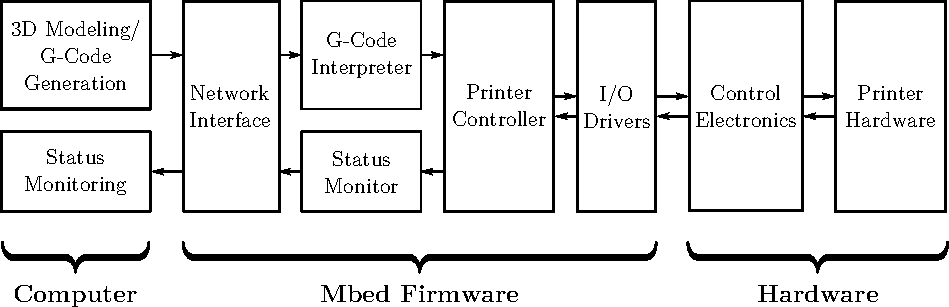
\includegraphics[width=1\textwidth]{diagrams/systemDiagramTop.pdf}
			% TODO: Explain what greyed out boxes mean.
			\caption{High-level diagram of overall system architecture.}
			\label{fig:systemDiagramTop}
		\end{figure}
	
	\section{Computer Software}
		
		This project is principally focused on the development of the firmware and
		electronics used by the printer. The process of generating 3D models and
		G-code is out of the scope of this project and will be carried out using
		off-the-shelf, open source tools.
		
		A limited amount of software will be provided which will allow G-code to be
		streamed to the printer and for the printer's status to be fetched.
	
	\section{Firmware}
		
		The microcontroller firmware will consist of three main components running
		on top of the FreeRTOS operating system (see Figure
		\ref{fig:systemDiagramFirmware}). The first will be the \uIP{} network stack
		for communication with the computer software. The second, is a G-code
		processing pipeline which will translate G-code into an appropriate sequence
		of commands to the electronics. The third component is a driver interface
		for the required components of the Mbed will be needed.
		
		\begin{figure}[here]
			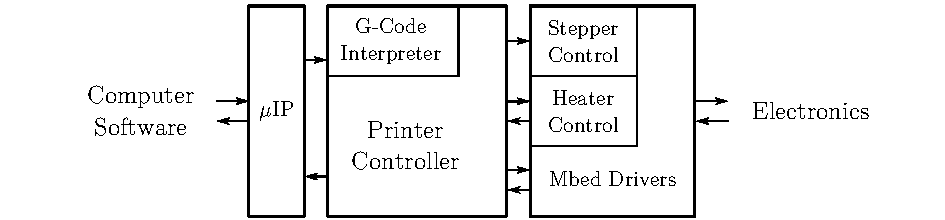
\includegraphics[width=1\textwidth]{diagrams/systemDiagramFirmware.pdf}
			\caption{Major components of the Mbed firmware}
			\label{fig:systemDiagramFirmware}
		\end{figure}
		
		\subsection{Network Interface}
			
			% XXX: This is probably not useful here
			
			The firmware will provide an interface for sending G-code and an interface
			for querying the printer's status.
			
			The G-code interface should be a simple open port which silently accepts
			and G-code streams and feeds them into the pipeline. It will need to
			support flow control as the rate at which the printer is able to accept
			G-code instructions will vary depending on what instructions are being
			executed. For example while waiting for heaters to warm up no instructions
			will be executed but during complex movements, many instructions may be
			executed in rapid secession. The interface must also be reliable. A
			missed, corrupted or out-of-order G-code instruction would cause
			unexpected results.
			
			% TODO: Cite G-code error checking
			
			TCP offers both reliable communication and flow control mechanisms and is
			implemented in \uIP{}.\footnote{Some G-code implementations have error
			checking and retransmission mechanisms but these are clunky and designed
			for use with serial connections. \cite{gcodeErrorChecking}} Unfortunately,
			the TCP flow-control implementation in \uIP{} was found to be buggy. Due
			to time constraints and the compact nature of \uIP{} a minimal custom
			UDP-based protocol should be used as a work-around.
			
			% XXX: Really mention UDP hack here?
			
			The status querying interface has few requirements and should be kept
			minimal to save microcontroller and development resources. A
			\verb+telnet+ compatible interface (which is both human and machine
			readable) should serve this purpose.
		
		\subsection{G-code Processing Pipeline}
			
			The main task of the firmware is to process incoming G-code from the
			network and to control the printer appropriately without stalling. A
			pipeline architecture (Figure \ref{fig:firmwarePipeline} was selected
			where G-code is buffered before being interpreted and converted into
			lower-level commands. The low-level commands are placed in a buffer and
			then executed in sequence to drive the printer.
			
			% XXX: Show data types on pipeline?
			\begin{figure}[here]
				
\includegraphics[width=1\textwidth]{diagrams/firmwarePipeline.pdf}
				\caption{G-code processing pipeline}
				\label{fig:firmwarePipeline}
			\end{figure}
			
			In order to reduce stalls due to data processing between commands the
			low-level commands used at the end of the pipeline exchange space for
			computation time by keeping all command arguments in formats directly used
			by the printer (e.g. distances in an integral number of steps and not
			floating point values in millimetres).
			
			Nearer the start of the pipeline, we want to minimise the effect of
			network latency by having a large buffer which gives the network time to
			respond to changes in the rate of command execution.
			
			% XXX: Mention relative buffer size:length ratios?
			
			Finally, by assigning a high priority to the Printer Controller we can
			minimise the latency between a command completing and another starting,
			especially during very short bursts of extremely detailed movements.
		
		\subsection{Drivers}
			
			In order to interface with the electronics and facilitate accurate timing
			various peripherals on the Mbed will require supporting driver code. In
			particular, the following features will be needed:
			
			\begin{description}
				\item[General-Purpose Input/Output (GPIO)]
					Allows TTL (Transistor-Transfer-Level) digital signals to be produced
					or read from the pins on the microcontroller. For example stepper
					control signals, end-stop signals.
				
				\item[Analog Input]
					Read analog signals from the electronics. For example readings from
					temperature sensors.
				
				\item[Timer]
					Produce interrupts at precisely timed intervals to allow stepper
					control signals to be produced.
				
				\item[Watch-dog Timer]
					To ensure fail-safe behaviour, a watch-dog timer can be used to reset
					and power down the system in the event of software malfunction.
			\end{description}
	
	\section{Hardware}
		
		\subsection{Microcontroller}
		
		\subsection{Stepper Control}
		
		\subsection{Heater \& DC Motor Control}
	
